\section{Overall system description}
A simplified class diagram describing the essentials of the system is shown in
figure \ref{fig:impl:sys:uml_complete}.

\begin{figure}[!htp]
\begin{center}
  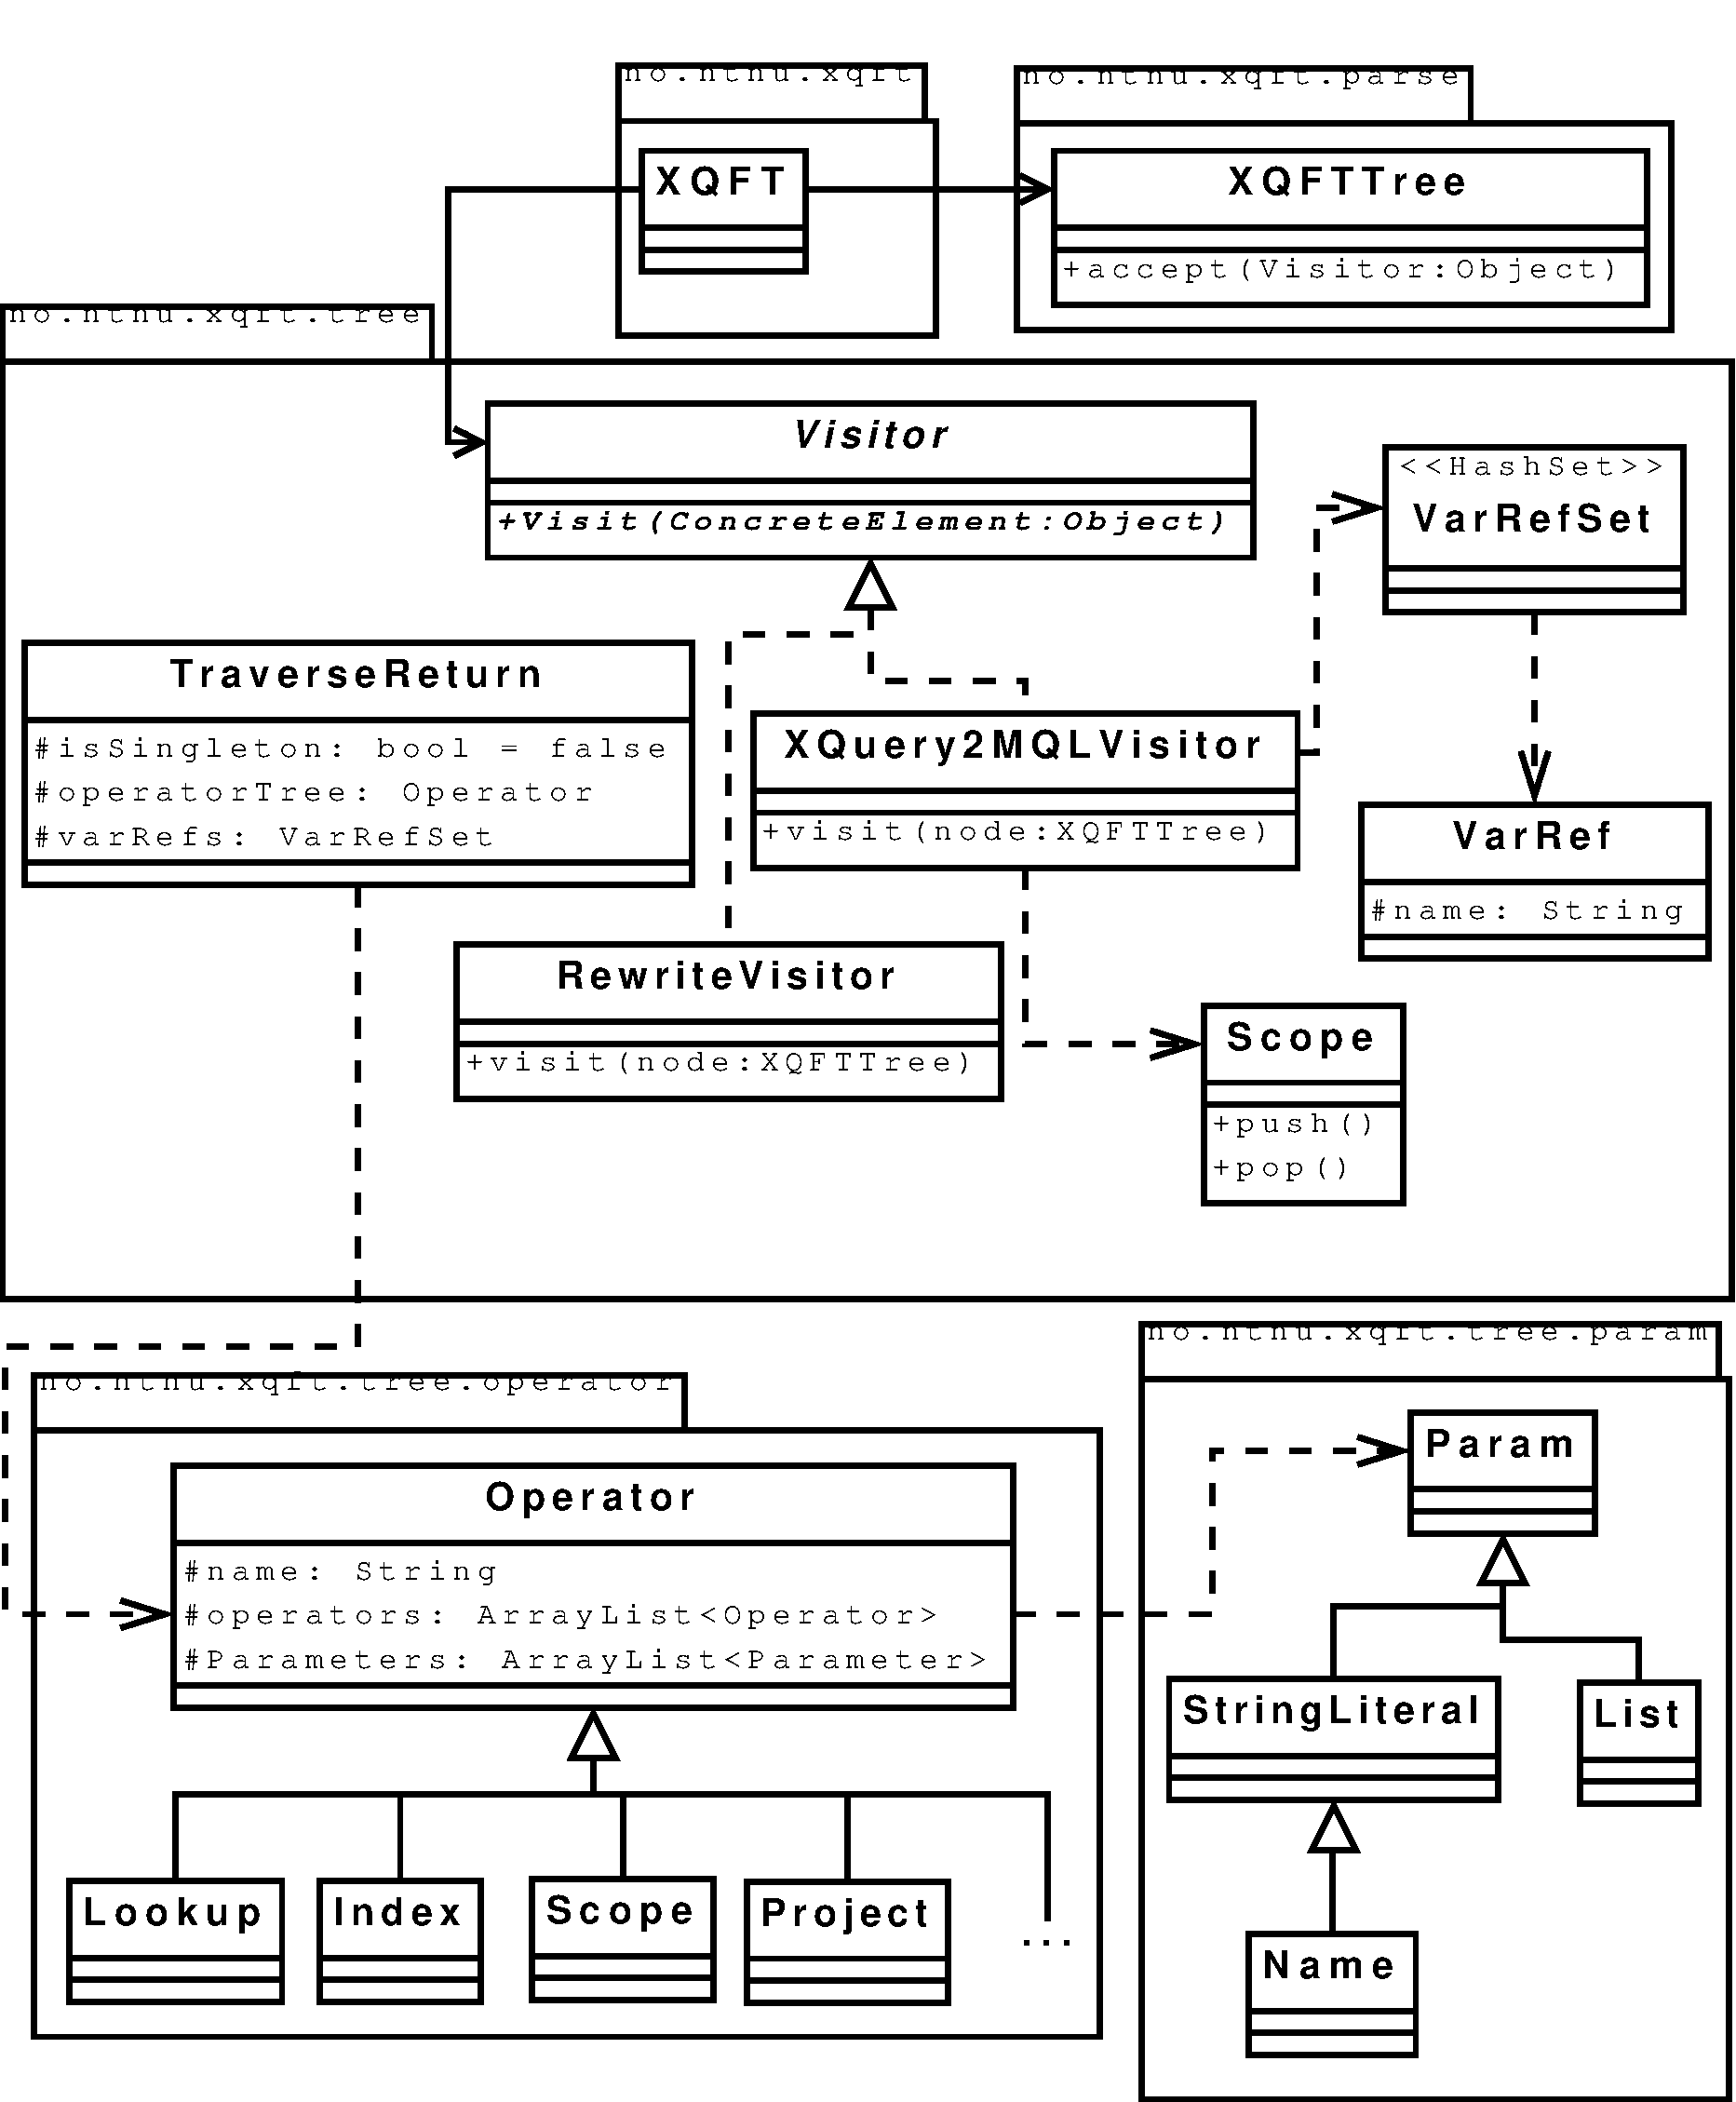
\includegraphics[scale=0.45]{diagrams/complete_uml}
  \caption{Simplified UML for complete implementation}
  \label{fig:impl:sys:uml_complete}
\end{center}
\end{figure}

\subsection{Data flow}
\begin{figure}[!htp]
\begin{center}
  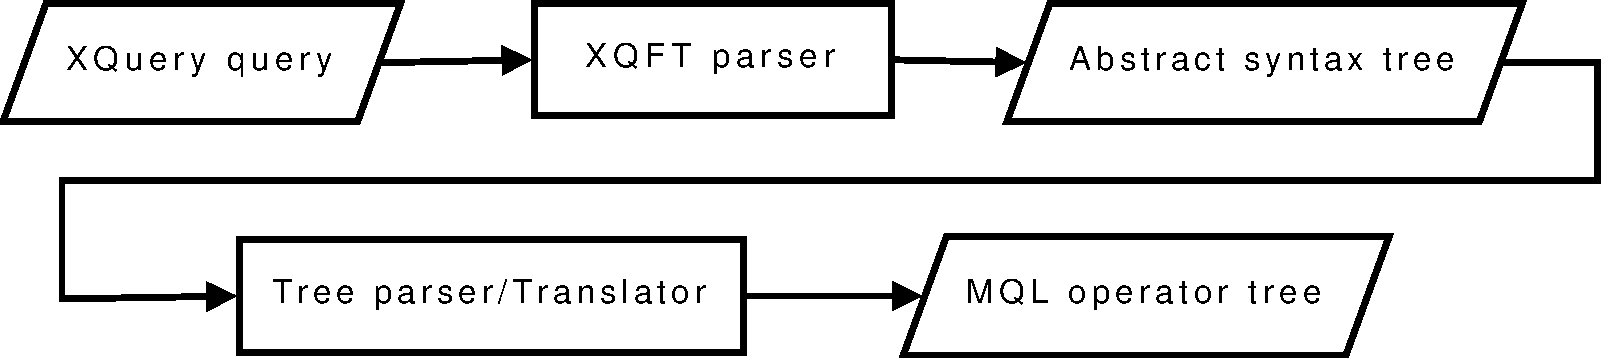
\includegraphics[scale=0.5]{diagrams/mql_dataflow}
  \caption{Data flow for XQuery parsing and translation to MQL}
  \label{fig:impl:sys:mql_dataflow}
\end{center}
\end{figure}
\subsection{Data flow}

\subsection{Visible external API}
\begin{itemize}
  \item Vise hvordan oversetteren kan brukes i sin helhet i andre programmer
\end{itemize}

\subsection{Command line interface}
\marginpar{\underline{\textbf{\Large TODO:}}\scriptsize ha det i appendix ala i fjor?}
Dette er ikke s\aa~veldig viktig \aa~skrive om, men greit \aa~ha med.
\begin{itemize}
  \item Argsengine
  \item Aksepterer flere strenger og filer
  \item Outputter til graphviz/dot og pdf, hvis tilgjengelig
  \item Dependencies (jar-filer og drit)
\end{itemize}